\section{Arsitektur Sistem}
Arsitektur sistem yang akan dibangun ditunjukkan pada gambar \ref{fig:arsitektur_sistem}. Komunikasi antara \textit{client} dengan server untuk proses pencarian data dilakukan secara asinkoron dengan menggunakan AJAX \textit{(Asynchronous Javascript and XML)}. Masing-masing ontologi yang akan dibangun diletakkan di lokasi yang terpisah yang nantinya dapat diakses melalui protokol http.

\begin{figure}[h]
    \centering
    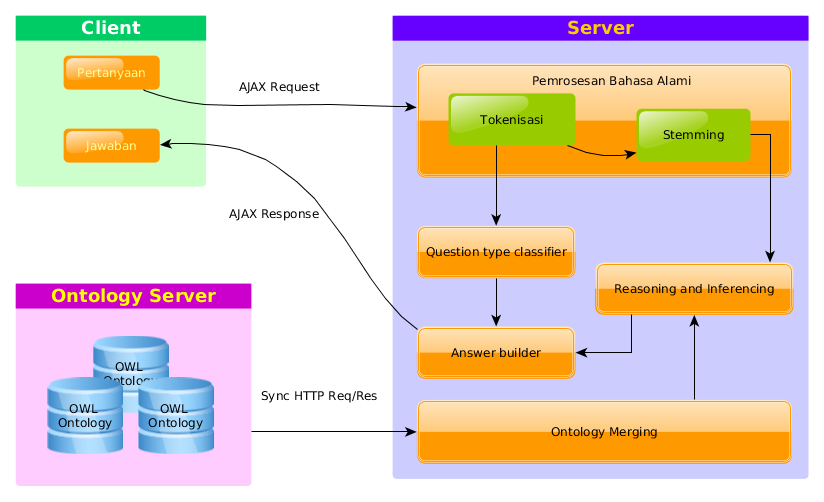
\includegraphics[width=1\textwidth]{arsitektur_sistem}
    \caption{Arsitektur sistem yang akan dikembangkan}
    \label{fig:arsitektur_sistem}
\end{figure}